\documentclass[11pt]{article}
\usepackage[a4paper,margin=21mm]{geometry}
\usepackage{graphicx}
\usepackage{hyperref}
\usepackage{longtable}
\usepackage{array}
\hypersetup{colorlinks=true,urlcolor=blue,linkcolor=blue}
\setlength{\parskip}{6pt}
\setlength{\parindent}{0pt}
\begin{document}
\begin{center}
{\LARGE Xedni affine-coset Lean review}\\[4pt]
{\large Technical packet, 2 November 2026}
\end{center}

\textbf{Scoped result.} For finite integer row and direction families, if each
direction annihilates every incidence row and is coordinatewise zero modulo
positive $q$, every integer recombination preserves those premises. Each
affine candidate $u+\sum_i c_iD_i$ has the same row dot products and residues
as $u$. Three named Lean declarations pass the pinned Lean 4.34.1 checker;
their axiom lists contain only \texttt{propext} and \texttt{Quot.sound}.

\begin{center}
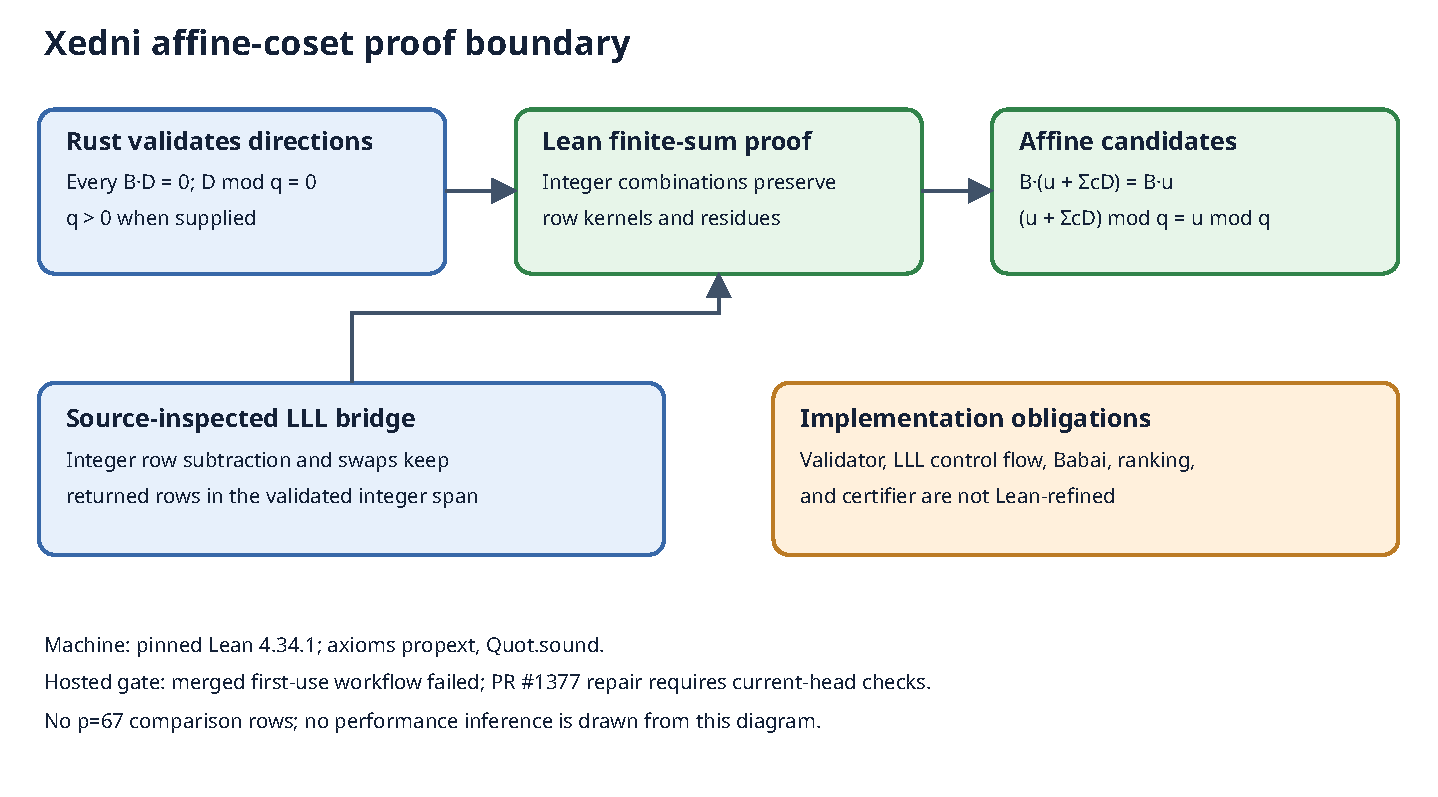
\includegraphics[width=0.98\linewidth]{proof-boundary.pdf}
\end{center}

\textbf{Independent review.} Blind algebra task \texttt{TASK-20261102-1a2b3c}
re-derived the finite-sum invariant without producer source, including
separate failed controls for the row-kernel and residue premises. Source task
\texttt{TASK-20261102-4d5e6f} traced the Rust validation, candidate loop,
integer LLL row operations, certifier, receipt, and workflow. Both filed
separate attestations; the shared independence checker found zero declared
violations after a documented cross-repository field-name adapter.

\textbf{Workflow finding and repair.} The original merged workflow at
cryptanalysis \texttt{749d807} failed on first-use elan setup even though Lean
returned zero. Repair PR
\href{https://github.com/isogeny-labs/cryptanalysis/pull/1377}{\#1377}
added explicit toolchain download and bound \texttt{lattice.rs} in the source
hash and workflow paths. All 28 applicable checks passed at head
\texttt{937b387}, including hosted Lean run
\href{https://github.com/isogeny-labs/cryptanalysis/actions/runs/41507496535}
{41507496535}. The repair merged as \texttt{15d5263}; its
\href{https://github.com/isogeny-labs/cryptanalysis/actions/runs/41510072421}
{main-push Lean run} passed. The earlier failure remains historical evidence.

\textbf{Claim separation.} The Lean algebra is machine checked and faithful
to the conditional candidate invariant. The Rust LLL span property is
source-inspected, not a formal refinement. Parser behavior, full validator
and LLL control flow, Babai choice, ranking, and certifier remain distinct
implementation obligations. The frozen $p=67$ diagnostic has no run rows
because checkpoint upload was denied, so no performance curve is inferred.

\textbf{Source bindings.} Producer commit \texttt{d243c3c}; Lean SHA-256
\texttt{c39148ea...e757}; Rust candidate SHA-256
\texttt{b08c9484...ac96}; LLL SHA-256 \texttt{0687b6c0...0b}.
The full hashes, per-claim table, controls, and report links are in the
adjacent \texttt{README.md}. The cross-field degree graph was checked against
its CSV and left unchanged because this proof changes no graph input.

\end{document}
